\chapter{Linked Connections}
\label{lc}

Linked Connections \cite{colpaert_iswc_2015} is een framework dat \textit{client-side} routeplanning mogelijk maakt. Alle algoritmen uit de literatuurstudie hebben als doel om een bepaalde server te lopen  waarboven een webservice gebouwd kan worden. CSA biedt een alternatieve oplossing op Dijkstra om routeplanning meer een datakarakter te geven. Linked Connections vervolledigt het dataprobleem door de intelligentie door te schuiven naar de cli\"ent. Volgende sectie de cli\"ent de snelste route kan berekenen.

\section{Principe}

Een Linked Connections server is verantwoordelijk voor het publiceren van connecties (zie \ref{probleemstelling}). Deze connecties worden door een Linked Connections cli\"ent opgevraagd om dan met CSA (zie \ref{csa}) een route te kunnen berekenen. De visie van Linked Data Fragments vertelt dat we een bepaalde selector op onze dataset moeten toepassen om de dataset in fragmenten in te delen. Dit laat toe om simpele webservers met intelligente cli\"ents te gebruiken. Een eenvoudige selector is de tijdsfunctie die connecties met een vertrektijd binnen een bepaald tijdsinterval beschouwt als een fragment. Zo'n fragment noemen we een \textit{basic Linked Connections fragment} (basis LCF). Met behulp van hypermedia-links (zie ook \ref{subsec:hypermedia}) worden deze fragmenten aan elkaar verweven. Dit laat toe dat de server de selector op de dataset dynamisch kan aanpassen, bijvoorbeeld van 10 minuten naar een halfuur afhankelijk van de hoeveelheid connecties binnen dat tijdsinterval. De Hydra-ontologie wordt gebruikt om de functionaliteit machine-verstaanbaar te maken. Figuur \ref{lcfragm} toont een overzicht hoe de connecties gepresenteerd worden door de server.

\begin{figure}[h!]
\centering
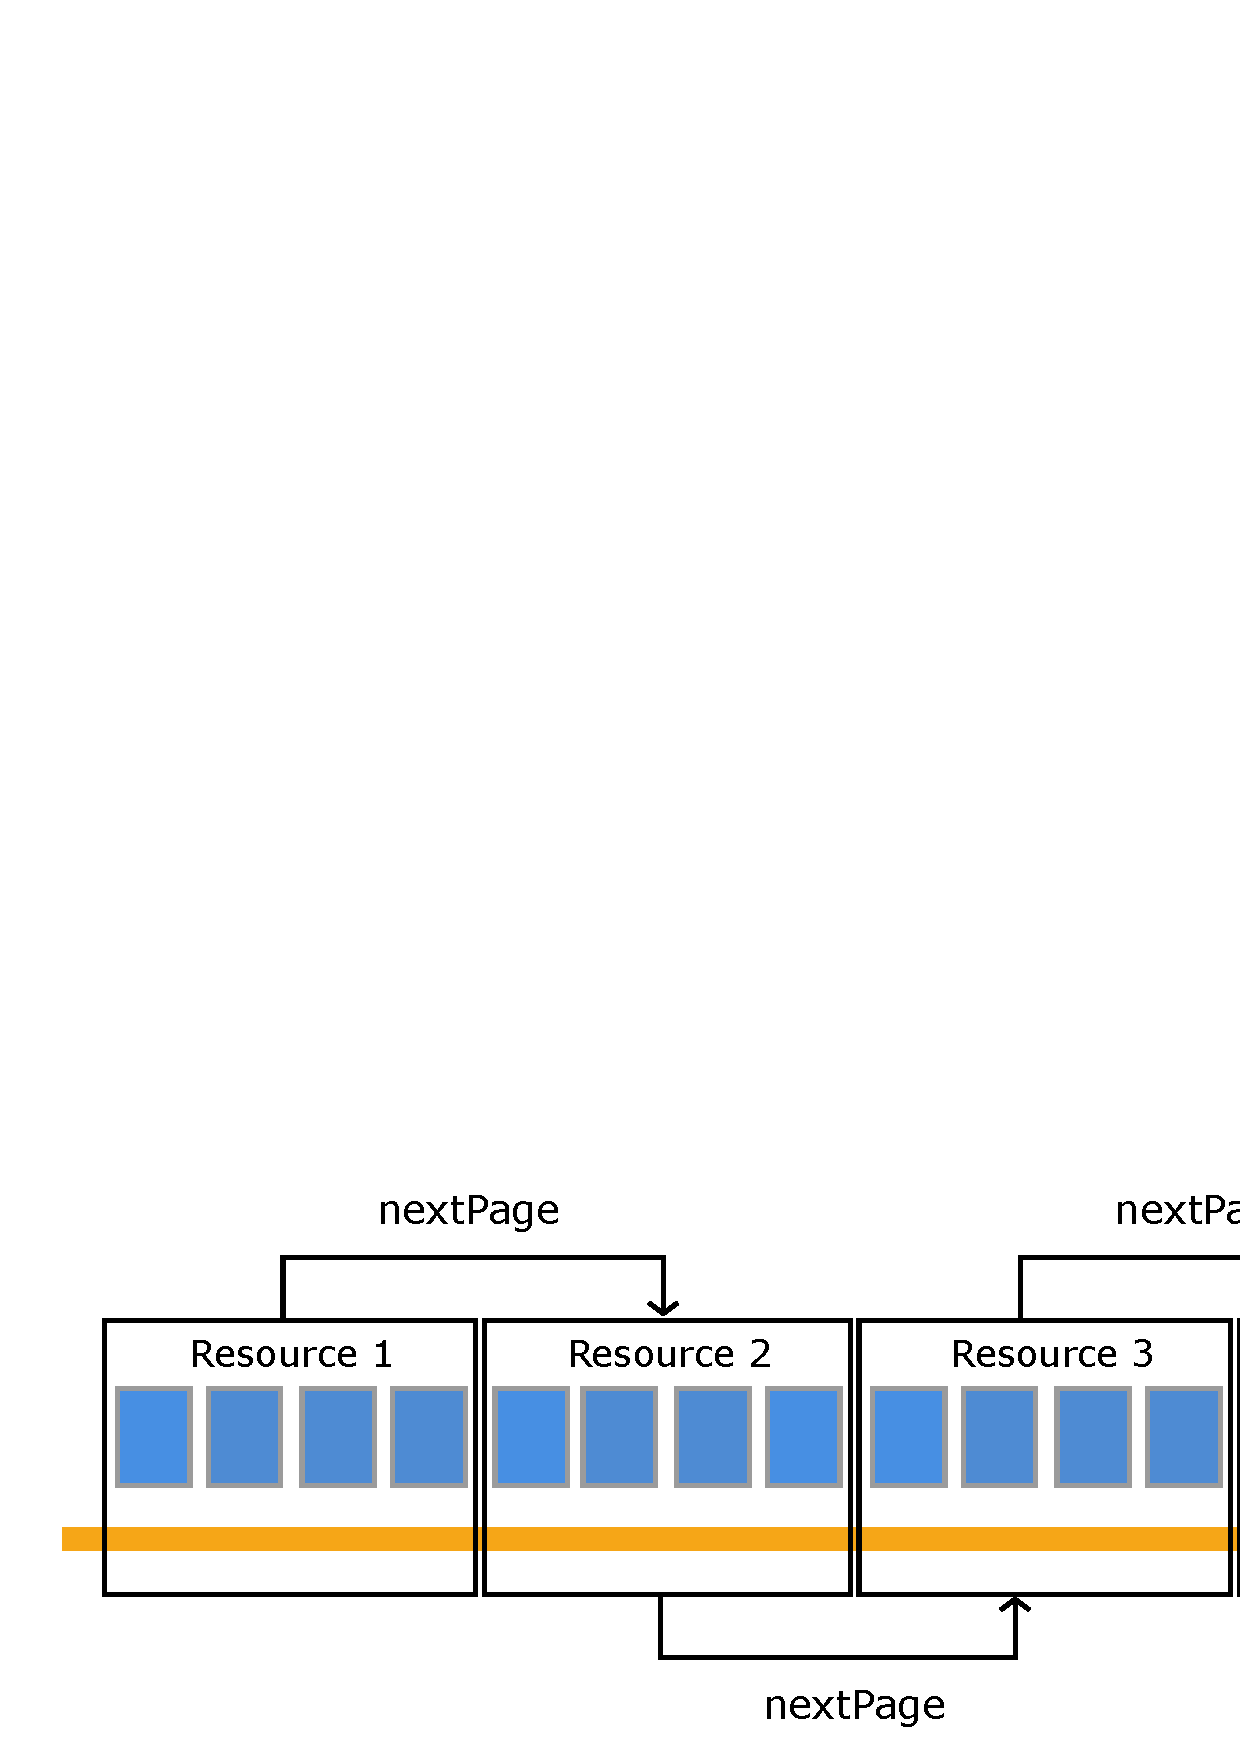
\includegraphics[width=0.8\textwidth]{hypermediafragmenten.png}
\caption{Connecties zijn onderverdeeld in fragmenten volgens een bepaald tijdsinterval, zogenaamde Linked Connections fragmenten. Met hydra:nextPage links kan makkelijk het volgende fragment gevonden worden.}
\label{lcfragm}
\end{figure}

De cli\"ent kan met behulp van textit{hydra:nextPage} links makkelijk het volgende fragment ophalen. De connecties van een fragment worden als invoer doorgegeven aan CSA (\ref{csa}). Deze bouwt een minimale overspannende boom met de snelste tijd om stops te bereiken. Wanneer het resultaat gevonden is, kan de cli\"ent stoppen met ophalen van fragmenten. Hieronder volgt een overzicht van de technologie\"en waarvan Linked Connections gebruik maakt.

\subsection{Technologie\"en}
Het publiceren van connecties gebeurt met behulp van drie technologie\"en: 
\begin{itemize}
\item De REST principes (zie ook \ref{rest}) worden gevolgd om ervoor te zorgen dat de fragmenten, de REST resources, cachebaar zijn. Er is namelijk een eindige verzameling URI's, afhankelijk van het ingestelde tijdsinterval. Listing \ref{queryconnecties} toont een template van deze REST interface.
\begin{lstlisting}[label=queryconnecties,caption=URI template van basis Linked Connections fragment.]
http://voorbeeld.org/connecties/?vertrekTijd=?
\end{lstlisting}
Als T het tijdsinterval in minuten is van de fragmenten, dan kan het aantal mogelijke URI's berekend worden met formule \ref{lc:aantalurisoorspronkelijk}. Is T=10min, dan zijn er 144 verschillende fragmenten.
\begin{equation} \label{lc:aantalurisoorspronkelijk}
24 * 60 / T
\end{equation}
De meeste publieke vervoersmaatschappijen rijden niet 24/24 dus in praktijk zijn er nog minder fragmenten. Met behulp van HTTP omleidingen kan dit opgelost worden.

\item Hypermedia zorgt niet enkel voor het vinden van volgende fragmenten, maar dient ook voor het voorzien van extra \textit{features} met Linked Data. Neem nu bijvoorbeeld een connectie. Deze heeft een bepaalde vertrek- en aankomststop. Er kunnen links toegevoegd worden die meer informatie geven over deze stops, bijvoorbeeld over vorm van de platforms of welke \textit{points of interest} er in de buurt zijn.

\item Het semantisch web zorgt voor de semantische interoperabiliteit van de gelinkte connecties en de hypermedia API. Gelinkte connecties maken o.a. gebruik van de GTFS \footnote{http://lov.okfn.org/dataset/lov/vocabs/gtfs} en Linked Connections\footnote{Linked Connections ontologie: http://semweb.mmlab.be/ns/linkedconnections} ontologi"en. De API functionaliteit maakt gebruik van de Hydra ontologie. Deze beschrijft dat de cli\"ent kan zoeken door de vertrektijd parameter in te vullen in de URI \textit{template}. Kortom, semantiek laat toe om generische clients te bouwen. 
Doordat zoveel mogelijk gebruik gemaakt wordt van Linked Data kan er gequery't worden over het web met bijvoorbeeld \textit{Triple Pattern Fragments} (TPF) (zie ook \ref{tpf}) Er bestaan al talrijke servers online die mogelijke uitbreidingen kunnen zijn. Met behulp van GeoNames \footnote{Momenteel is er al een TPF-server met gelinkte GeoNames beschikbaar: http://data.linkeddatafragments.org/geonames} kan er meer informatie gevonden worden over bepaalde geolocaties. Ook voor \textit{Points of Interest} is een Linked Data portaal te vinden. \footnote{Ook hiervoor is een Linked Data portaal aanwezig die door intelligente cli\"ents gebrowset kunnen worden: http://data.linkeddatafragments.org/linkedgeodata}.
\end{itemize}

\subsection{Basic Linked Connections Fragments}
\label{blcf}
Basic LCF zijn fragmenten met connecties die onderverdeeld zijn met de vertrektijd tussen een bepaald tijdsinterval. Het kost de server weinig moeite om data te publiceren door de hoge cachebaarheid. Een cli\"ent moet daarentegen veel connecties scannen om tot een route te komen. In hoofdstuk \ref{resultaten-origineel} zal de exacte performantie van routeplanning met deze fragmenten verduidelijkt worden.

\begin{figure}[h!]
\centering
\includegraphics[width=0.8\textwidth]{LDF-as5.png}
\caption{Linked Data Fragmenten-as met Linked Connections}
\label{ldf-lc5}
\end{figure}

In volgende sectie bespreken we hoe connecties in deze masterproef gegenereerd zijn.

\section{Convertor naar connecties}

Door het wereldwijde gebruik van GTFS hebben we in deze masterproef toegespitst op het converteren van een GTFS \textit{feed} naar connecties. Doordat meerdere bestanden tegelijk behandeld moeten worden, werd er in de ontwerpfase beslist om met een databank te werken. Het is belangrijk op te merken dat connecties niet gesorteerd moeten zijn. Deze worden later in de databank van een Linked Connections server ingeladen die zelf sorteert tijdens het query'en. 

Figuur \ref{inladengtfs} toont een globaal overzicht om connecties te genereren. De eerste stap bestaat uit het inladen in een MySQL-databank. Daarna worden connecties met PHP scripts gegenereerd en weggeschreven naar een apart bestand. In volgende subsectie gaan we dieper in de logica om connecties te genereren met queries.

\begin{figure}[h!]
\centering
\includegraphics[width=0.7\textwidth,scale=1.0]{Preprocessor.png}
\caption{Overzicht hoe connecties worden gegenereerd uit een GTFS feed. Deze wordt ingeladen in een MySQL databank. Met de scripttaal PHP worden connecties gegenereerd.}
\label{inladengtfs}
\end{figure}

\subsection{Connectiescript}

Nadat de bestanden van een GTFS feed in gelijknamige tabellen van databank ingeladen zijn, kan het genereren van connecties starten. Deze connecties worden dag per dag berekend. Ofwel worden start- en einddatum meegegeven als parameters, ofwel worden start- en einddatum van de GTFS feed  genomen. 

\begin{figure}[h!]
\centering
\includegraphics[width=1.0\textwidth]{volgordeconvertor.png}
\caption{Per dag worden de corresponderende service ID's, trip ID's en route ID's berekend. De vertrek-/aankomststopplaats met respectievelijk vertrek-/aankomsttijd worden berekend uit een verzameling stoptimes. }
\end{figure}

Een connectie vereist informatie uit verschillende tabellen. Deze moeten per dag $d$ stapsgewijs opgehaald worden:

\begin{enumerate}
\item Een eerste stap is het ophalen van alle services die actief zijn op $d$. Deze services zitten in de \textit{calendar} en \textit{calendar\_dates} tabellen.
\item De \textit{trips} tabel bevat de mapping tussen een service, route en trip. Voor elke service komt overeen met een route en meerdere trips. Een route is niet essentieel voor een connectie, maar bevat wel interessante informatie zoals de routebeschrijving en type voertuig.
\item De laatste stap is het overlopen van \textit{stoptimes.txt}. Voor elke trip komt een reeks stoptijden overeen. Uit de combinatie van twee opeenvolgende stoptijden van eenzelfde trip wordt een connectie berekend. Lijst \ref{vbstoptimes} bevat een voorbeeld van twee opeenvolgende stoptijden van een bepaalde trip. De vertrektijd en vertrekstop van een eerste stoptijd wordt samengenomen met de aankomsttijd en aankomststop van de tweede stoptijd. 

\begin{lstlisting}[label=vbstoptimes,caption=Voorbeeldstoptijden uit GTFS \textit{stop\_times.txt}.]
trip_id,arrival_time,departure_time,stop_id,stop_sequence
16,07:18:00,07:18:00,8200100,1
16,07:33:00,07:33:00,8200110,2
\end{lstlisting}

Hiermee zijn alle stappen doorlopen en kan een connectie weggeschreven worden. Codevoorbeeld \ref{connectiejsonld} toont hoe een connectie eruit ziet bij output. Merk op dat een '@context' niet is toegevoegd en de connectie ook niet in een graaf zit. In subsectie \ref{jsonldstream} wordt hierover meer uitleg gegeven.

\begin{lstlisting}[label=connectiejsonld,caption=Voorbeeld van een connectie voor een bepaalde trip in JSON-LD formaat.]
{	
	"@id": "http://example.org/connections/1"
	"@type": "http://semweb.mmlab.be/ns/linkedconnections#Connection",
	"http://vocab.gtfs.org/terms#trip": "16",
	"http://vocab.gtfs.org/terms#route": "route-1",
	"http://semweb.mmlab.be/ns/linkedconnections#departureTime": "2015-10-21T06:18:00.000Z",
	"http://semweb.mmlab.be/ns/linkedconnections#departureStop": "8200100",
	"http://semweb.mmlab.be/ns/linkedconnections#arrivalTime": "2015-10-21T06:33:00.000Z",
	"http://semweb.mmlab.be/ns/linkedconnections#arrivalStop": "8200110"
}
\end{lstlisting}
\end{enumerate}

Als je tijd van de stoptijden in \ref{vbstoptimes} vergelijkt met de aankomst- en vertrektijd in de connectie \ref{connectiejsonld} zie je dat de tijd in de connectie een uur vroeger is. Dit komt doordat de tijd van connecties in Coordinated Universal Time (UTC) staat. Dit is herkenbaar aan de 'Z' die vanachter staat. Er moet altijd rekening gehouden worden met de tijdszone van waar de GTFS feed zich afspeelt. Het voorbeeld van \ref{vbstoptimes} stelt een feed uit Belgi\"e voor in wintertijd. Belgi\"e volgt in de wintertijd UTC+1 en in de zomertijd UTC+2. Er moet dus een uur afgetrokken in deze periode om een correcte UTC tijd te bekomen.

Een van de moeilijkheden voor het genereren van connecties was het ophalen van trips die over meerdere dagen actief zijn. GTFS lost dit op door de tijd na middernacht op te tellen bij 24u, bijvoorbeeld 2u 's nachts staat weergegeven als 26u. Volgens GTFS rijden deze stoptimes allemaal op dezelfde dag, maar voor Linked Connections zijn dit effectief twee verschillende dagen, omdat er met exacte tijden gewerkt wordt. Het script moet dus bij de startdatum rekening houden met trips van de dag ervoor die na middernacht nog actief zijn.
Om dit op te lossen werden er twee extra vlaggen toegevoegd in de databank of de vertrek- en aankomsttijd van een stoptijd voor of na middernacht plaatsvinden. Met aparte queries kunnen de stoptijden na middernacht opgevraagd worden.

Een databank gebruiken heeft als grote nadeel dat de data ingeladen moet worden vooraleer berekeningen kunnen plaatsvinden. In \ref{table:inladengtfs} staat een overzicht van de drie gebruikte datasets in deze masterproef met de tijd om in te laden. Voor zeer grote datasets, zoals De Lijn, is inladen een bottleneck.

\begin{table}[htbp]
\centering
\begin{tabular}{ | l || c | c | c |}
  \hline			
    & Tijd inladen (min) & Grootte (MB) & Periode (weken) \\ \hline
  NMBS & 3.1 & 1.1 & 12  \\
  NS & 8.35 & 21.4 & 56 \\
  De Lijn & 100 & 44 & 10 \\
  \hline  
\end{tabular}
\caption{Tijd om een GTFS feed in te laden in een MySQL databank.}
\label{table:inladengtfs}
\end{table}

Het genereren van connecties zelf gaat een stuk rapper. In \ref{table:connectiesgenereren} zie je dat voor kleine datasets (zoals NMBS en NS) het minder dan minuut duurt om de connecties voor een dag te berekenen. De Lijn scoort opnieuw zeer slecht door de grootte van de dataset.

\begin{table}[htbp]
\centering
\begin{tabular}{ | l || c | c | c | c |}
  \hline			
    & Connecties & Aantal stops & Tijd (min) & Tijd met nieuwe convertor (min) \\ \hline
  NMBS & 55479 & 597 & 0.21 & \\
  NS &  41796 & 2531 & 1.30 & \\
  De Lijn & 1049186 & 35275  & 14.97 & \\
  \hline  
\end{tabular}
\caption{Tijd om connecties te genereren voor een dag.}
\label{table:connectiesgenereren}
\end{table}

Ondertussen is er een veel snellere convertor \footnote{Zie: github.com/linkedconnections/gtfs2lc} gemaakt die connecties zonder databank kan genereren. In de laatste kolom van \ref{table:connectiesgenereren} staat de tijd met de nieuwe convertor vermeld. Deze werkt veel sneller en heeft geen bottleneck meer.

Connecties worden een per een weggeschreven naar een apart bestand. Hiervoor wordt er gebruik gemaakt van een nieuwe specificatie, genaamd \textit{JSON-LD stream}.

\subsection {JSON-LD stream}
\label{jsonldstream}
Om connecties als Linked Data te publiceren werd er voor gekozen om JSON-LD te gebruiken. JSON wordt beschouwt als het \textit{de facto} dataformaat op het web dankzij de compactheid, leesbaarheid en vele handige tools die hiervan gebruik maken. Wanneer een verzameling objecten dezelfde context heeft, zijn er twee mogelijkheden om deze te publiceren:
\begin{itemize}
\item een gemeenschappelijke context voorzien en alle objecten in bijhorende graaf steken (zie \ref{tripjsonldgraph}). Deze methode vereist dat de graaf in het geheugen geladen moet worden vooraleer verdere operaties mogelijk zijn.
\item elk object een context geven (zie \ref{tripjsonld}). Met deze methode kan object per object gestreamt worden, maar zorgt voor grote overhead door de context die telkens mee gepubliceerd wordt.
\end{itemize}
Een oplossing hiervoor is de JSON-LD streamspecificatie \footnote{Zie: https://github.com/pietercolpaert/jsonld-stream}. Deze geeft aan dat een context van een object impliciet van toepassing is op alle andere objecten van hetzelfde document. Zo moet er maar eenmalig een context opgegeven worden.
De voorbewerker kan volgens dit formaat connecties als Linked Data wegschrijven zonder extra data in het geheugen te moeten houden. Dit stroomlijnen is belangrijk om de data later lijn per lijn te kunnen inladen in de databank van een LC server.

Vooraleer we intermodaliteit bekijken, bespreken we eerst hoe een Linked Connections cli\"ent aangemaakt kan worden.

\section{Cli\"ent}

De cli\"ent is verantwoordelijk voor het berekenen van de snelste route met CSA. Deze kan met een paar lijntjes code aangemaakt worden (zie \ref{clientvb}).
\begin{lstlisting}[label=clientvb,caption=Code om een LC cli\"ent op te zetten in JavaScript.]
var planner = new window.lc.Client({"entrypoints" : ["http://example.linkedconnections.org/"]});
planner.query({
			"departureStop": "Brussel-Zuid",
			"arrivalStop": "Gent-Sint-Pieters",
			"departureTime": new Date("2015-11-05T10:00")
			}, function (stream) {
				stream.on('result', function (pad) {
					// pad bevat verzameling connecties die snelste route voorstellen
				});
			 	stream.on('data', function (connectie) {
			 		// connectie is gebruikt geweest voor minimale overspannende boom
			 	});
});
\end{lstlisting}
\label{vbclient}

Er zijn twee fases vooraleer routes effectief berekend kunnen worden:

\begin{itemize}
\item Configuratiefase: de LC client moet weten welke servers er bereikt moeten worden door de webadressen toe te voegen in de \textit{entrypoints}-rij. Ook moet de query ingesteld worden. Momenteel wordt enkel het startpunt, aankomstpunt en vertrektijd ondersteund.
\item Nadat de planner ge\"initialiseerd is, zal deze connecties opvragen en doorgeven aan CSA. CSA stuurt zelf notificaties wanneer een bepaalde actie ondernomen is. Zo wordt de \textit{data}-notificatie uitgestuurd wanneer een connectie gebruikt is voor de minimale overspannende boom.
\end{itemize}

Momenteel is er enkel ondersteuning om een connectiestroom van een \textit{entrypoint} op te vragen. Andere implementaties die van CSA gebruik maken, houden alle connecties bij in een server. De bedoeling van Linked Connections is om schaalbaar verschillende servers te kunnen opzetten voor elke modi en/of land. Figuur \ref{overzichtclientserver} toont een overzicht van een opstelling met meerdere servers. Rechts staan twee servers, de ene verantwoordelijk voor busdata, de andere voor treindata.

% todo: simpeler maken!
\begin{figure}[h!]
\centering
\includegraphics[width=0.5\textwidth]{OverzichtClientServer.png}
\label{overzichtclientserver}
\caption{Opstelling van een client en twee Linked Connections servers die elk verantwoordelijk zijn voor een modi.}
\end{figure}

CSA verwacht als invoer een gesorteerde rij van connecties. Elke connectiestroom van een server is zelf gesorteerd, maar niet onderling.  De \textit{merger} die hiervoor zorgt, wordt in volgende sectie besproken.

\subsection{Merger}

Een merger zorgt ervoor dat een of meerdere gesorteerde connectiestromen dynamisch samengevoegd kunnen worden. Het resultaat is een connectiestroom die zelf ook gesorteerd is op vertrektijd. Met dynamisch wordt bedoeld dat de cli\"ent op elk moment kan beslissen om connectiestromen toe te voegen of te verwijderen.

Connecties komen onder de vorm van een \textit{stream} binnen. Een \textit{stream} verwerkt data en stuurt deze door met notificaties. Deze notificaties worden opgevangen door notificatieluisteraars. Dit werkt op een asynchrone manier waardoor het niet vanzelfsprekend is om aan de sorteringsvoorwaarde te voldoen. De volgorde waarin deze notificaties worden opgeworpen is onvoorspelbaar waardoor een een mechanisme ontworpen moet worden om te verzekeren dat elke stroom aan bod is gekomen.
 
Figuur \ref{merger} toont een overzicht van een merger. De merger luistert (1) naar de verschillende onderling gesorteerde datastromen. Wanneer er data vrijgeven wordt, wordt dit toegevoegd aan een van de wachtrijen (2). Deze wachtrijen hebben als voorwaarde dat ze zelf gesorteerd zijn.

\begin{figure}[h!]
\centering
\includegraphics[width=0.5\textwidth]{merger.png}
\caption{Overzicht merger}
\label{merger}
\end{figure}

Om te kunnen garanderen dat de totale connectiestroom (3) gesorteerd is, wordt er vereist dat de wachtrijen connecties bevatten van elke connectiestroom (1). Doordat de stromen asynchroon werken, moet elke stroom telkens gepauzeerd worden. Nadat elke stroom data heeft vrijgegeven kan de merger connecties teruggeven (3) met dezelfde vertrektijd. Deze minimale vertrektijd wordt apart bijgehouden. Wanneer alle connecties met deze minimale vertrektijd verwerkt zijn, wordt deze ge\"updatet.
Een andere reden waarom de datastromen telkens worden gepauzeerd is door het feit dat de cli\"ent beslissingstijd moet hebben. Zo kan er op elk moment beslist worden om een bepaalde connectiestroom uit te schakelen of toe te voegen. Een use case zou het toevoegen zijn van busdata wanneer het doel binnen een bepaalde straal bereikbaar is.

Listing \ref{vbmerger} toont hoe een merger ge\"initialiseerd kan worden. Merk op dat bij elke connectiestroom een naam toegevoegd is. Zo kan de merger controlleren dat er voor elke stroomminstens een connectie in de wachtrijen aanwezig is. De cli\"ent kan hiermee ook gemakkelijk acties ondernemen. Zo kan vanaf een bepaald moment beslist worden om een connectiestroom toe te voegen aan de merger.

\begin{lstlisting}[label=vbmerger,caption=Voorbeeldcode van een merger. Deze voegt meerdere stromen van connecties samen.]
"var connectionsStreams = [
    [ 'stream1', connectionsReadStream1 ],
    [ 'stream2', connectionsReadStream2 ],
    ...
];

var connectionsReadStream = new MergeStream(connectionsStreams, query.departureTime);

connectionsReadStream.on("data", function (connection) {
    connectionsReadStream.addConnectionsStream('busStroom', newConnectionsReadStream);
});"
\end{lstlisting}

\section{Conclusie}

We hebben gezien hoe connecties gegenereerd kunnen worden uit een GTFS feed en hoe een Linked Connections server deze als \textit{basic LC fragments} aanbiedt aan de cli\"ent. Deze laatste maakt dan gebruik van CSA om de snelste route te berekenen. Een eerste stap naar intermodaliteit werd gezet door de introductie van een merger van connectiestromen.

In volgend hoofdstuk onderzoeken we hoe snel deze opstelling werkt voor een of meerdere datasets.

%\subsection{Voor- en nadelen}
%
%\begin{itemize}
%\item Routeplanning is een dataprobleem geworden. Datapubliceerders zijn verantwoordelijk voor het publiceren van connecties en bijhorende data. Zo kan er makkelijk data toegevoegd worden via hypermedia: \textit{point of interests}, rolstoelvriendelijkheid etc. De cli\"ent bepaalt zelf welke informatie deze wil gebruiken.
%\item Connecties zijn makkelijk distribueerbaar over meerdere servers.
%\end{itemize}